\documentclass{article}
\usepackage{amsmath}
\usepackage{graphicx}
\usepackage{lettrine}
\usepackage{hyperref}

\begin{document}


\begin{titlepage}
    \centering
    \vspace*{1cm}
    
    \Huge
    \textbf{Planes and Birds: Minimizing energy}
    
    \vspace{0.5cm}
    
    \Large
    Tao Su
    \vspace{1.5cm}

    \large 
    \textit{HornorsCalc1 Fall 2024 Project Final}
    \vfill

    \begin{figure}[h]
        \centering
        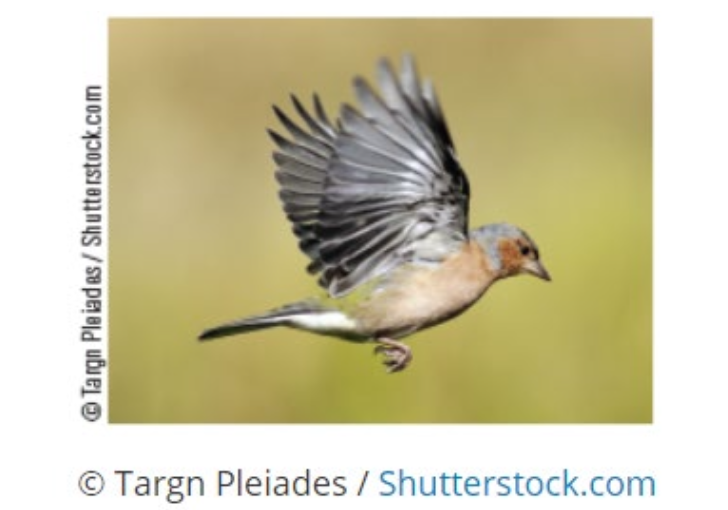
\includegraphics[width=1\textwidth]{coverPage.png}
        \caption{\small A flying Bird}
        \label{fig:cover}
    \end{figure}
            
    \Large
    \today  % or you can replace with a specific date
    
\end{titlepage}

\newpage

\subsection*{The Introduction}


\lettrine[lines=2]{S}{mall} birds, such as finches, alternate between flapping their wings and gliding, a behavior essential to managing energy during flight. This project focuses on the relationship between a bird’s flight speed, the power required, and the average energy consumed, exploring how different speeds impact energy efficiency.

The analysis uses calculus, particularly derivatives, to examine how variations in speed affect both power and energy expenditure. By calculating the rate of change in power requirements with respect to speed, we aim to determine optimal flight conditions that minimize energy use.

This approach draws on principles similar to those for fixed-wing aircraft, where energy and power requirements are essential to understanding flight dynamics. This project applies mathematical analysis to a biological context, using derivatives to derive meaningful insights about energy efficiency in bird flight.

Through this study, we aim to gain a deeper understanding of the mathematical relationships governing flight, which aligns with the course objectives of applying calculus to real-world phenomena and deepening our understanding of energy optimization in dynamic systems.
\newpage


\subsection*{Part 1:}
\begin{figure}[h]
    \centering
    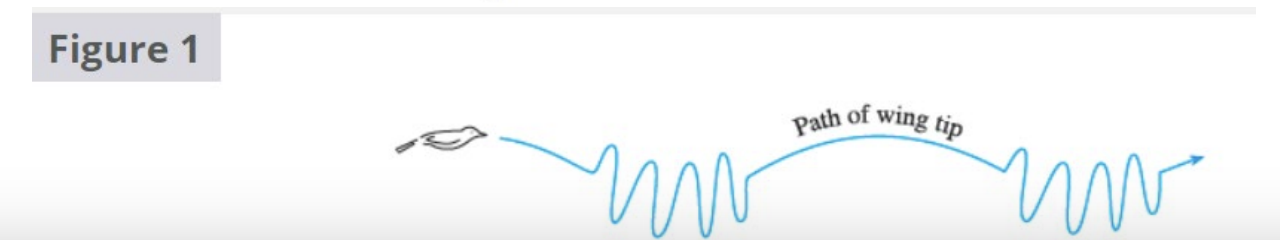
\includegraphics[width=0.5\textwidth]{bird.png}
    \caption{\small The trajectory of a flying bird.}
    \label{fig:bird}
\end{figure}

The power needed to propel an airplane forward at velocity \( v \) is: 
\[
P = Av^3 + \frac{BL^2}{v}.
\]
where \( A \) and \( B \) are positive constants specific to the particular aircraft, and \( L \) is the lift—the upward force supporting the weight of the plane (or bird).
\setlength{\parskip}{2em}

To determine the relationship between the power \(P\) and the speed \(v\), we can start with finding the derivative of \(P'\) with respect to \(v\).

The derivative of \( P \) with respect to \( v \) is:
\[
P'(v) = 3Av^2 - \frac{BL^2}{v^2}.
\]

To find the critical point of \( P(v) \), we set \( P'(v) = 0 \):
\[
P'(v) = 3Av^2 - \frac{BL^2}{v^2} = 0.
\]
Solving for \( v \), we get:
\[
v^4 = \frac{BL^2}{3A}.
\]
Therefore, we can find the speed \( V \) as:
\[
V = \sqrt[4]{\frac{BL^2}{3A}}.
\]

To determine whether this speed represents a minimum or maximum, we test the second derivative:
\[
P''(v) = 6Av + \frac{2BL^2}{v^3}.
\]

Since \( A \) and \( B \) are positive constants, and \( L^2 \) and \( v \) are always positive, we find that:
\[
P''(v) = 6Av + \frac{2BL^2}{v^3} > 0.
\]

Thus, when \( P'(v) = 0 \) and \( P''(v) > 0 \), \( P \) concaved up, indicating an absolute minimum. Therefore, when
\[
\text{the speed } V \text{ when power } p \text{ is minimized }  V_p = \sqrt[4]{\frac{BL^2}{3A}}
\]
the required power \( P \) is minimized.

\subsection*{Part 2:}
The speed found in Part 1 minimizes power, but a faster speed might use less fuel. The energy needed to propel the airplane/bird a unit distance is \( E = \frac{P}{v} \). At what speed is energy minimized?

To find out the answer, we first need to know the relationship between \( E \) and \( v \). 

Fortunately, we know:
\[
P = Av^3 + \frac{BL^2}{v} \text{ from the beginning, and }
E = \frac{P}{v}
\]

So, we can easily derive the equation for \( E(v) \):
\[
E(v) = Av^2 + \frac{BL^2}{v^2}
\]
Next, let's take the derivative of \(E\) respect to \(v\):
\[
E'(v) = 2Av-\frac{2BL^2}{v^3}
\]
Same as part 1, we also need to find the critical point of \(E'(v)\):
\[\text{We set } E'(v) = 2Av-\frac{2BL^2}{v^3} = 0,\]
\[\text{ solve for }v, v^4=\frac{2BL^2}{2A}, v = \sqrt[4]{\frac{BL^2}{A}},\text{ and }V > 0.\]
Then we take the second derivative of \(E'\) respect to \(v\):
\[E''(v) = 2A + \frac{6BL^2}{v^4},
\text{ because } 2A > 0, \text{ and } \frac{6BL^2}{v^4} > 0, E''(v) > 0.\]
Therefore,
 \[\text{when the speed }V_e = \sqrt[4]{\frac{BL^2}{A}}, E\text{ has the absolute minimum,}\]
  the energy is minimized.

\subsection*{Part 3:}
How much faster is the speed for minimum energy than the speed for minimum power?
\setlength{\parskip}{1em}

By observation, we found that both \(V_p\)(the speed \(V\) when power \(p\) is minimized) and \(V_e\) (the speed \(V\) when energy \(e\) is minimized) are 4th root, therefore, we can compare these two value by dividing \(V_e\) by \(V_p\):
\[\frac{V_e}{V_p}=\frac{\sqrt[4]{\frac{BL^2}{A}}}{\sqrt[4]{\frac{BL^2}{3A}}} = \sqrt[4]{3}\]

Therefore, we can conclude that, the speed \(V_e\) for minimum energy is \(\sqrt[4]{3}\) times faster than the speed for minimum power \(V_p\).

\subsection*{Part 4:}
\label{sec:part4}
In applying the equation of Part 1 to bird flight we split the term \(Av^3\)into two
parts: \(A_bv^3\) for the bird’s body and \(A_wv^3\) for its wings. Let \(x\) be the fraction of flying time spent in flapping mode. If \(m\) is the bird’s mass and all the lift occurs during flapping, then the lift is \(\frac{mg}{x}\) and so the power needed during flapping is:
\[P_\text{flap} = (A_b+A_w)v^3+\frac{B(\frac{mg}{x})^2}{v}\]
The power while wings are folded is \(P_\text{fold}=A_bv^3\). Show that the average power over an entire flight cycle is:
\[\overline{P}=P_\text{flap}+(1-x)P_\text{fold} = A_bv^3+xA_wv^3+\frac{Bm^2g^2}{xv}\]

To address this problem, first, let's break it down:

 The energy \(E\) for the whole cycle is actually generated by bird flapping its wings during the time of flapping stage, afterward, the bird stops flapping and folds its wings.

 But birds keeps flying, more acurately, it keeps gliding, during the time of folding stage, bird doesn't spend more energy, instead, it uses the remaining energy from the flapping stage.

Therefore, the total energy during the whole flying process is qual to the energy during flapping, and by the physics definition, the relationship between power \(P\) and energy \(E\) is:
\[\overline{P}=\frac{\Delta E}{\Delta t}\]
And the time during flapping is fraction \(x\), then the time during folding would be \(1-x\), therefore:
\[\text{the energy spends during flapping is } E_\text{flap} =P_\text{flap}\times  x \]
\[\text{the energy spends during folding is } E_\text{fold} = P_\text{fold}\times (1-x)\] 
\[\text{the total energy spent during the flying cycle would be: }E = E_\text{flap} +E_\text{fold} \]
And then,let's come back to the definition of power:
 \[\overline{P}=\frac{\Delta E}{\Delta t}=\frac{E}{x+(1-x)}=P_\text{flap} + P_\text{fold}\]
 Therefore:
\[\overline{P}=P_\text{flap}+(1-x)P_\text{fold} = A_bv^3+xA_wv^3+\frac{Bm^2g^2}{xv}\]
Thus, we proved the hypothesis of average power during each flying cycle.


\subsection*{Part 5:}
For what value of \(x\) is the average power a minimum?
\setlength{\parskip}{1em}

We've got the average power \(\overline{P}\) from the part 4, then let's take the derivative of \(\overline{P}\) respect to \(x\):
\[\overline{P}\text{ }'(x)= A_wv^3-\frac{Bm^2g^2}{x^2v}\]
and its second derivative:
\[\overline{P}\text{ }'' = \frac{Bm^2g^2}{x^3v}\]
We found that, the second derivative of \(\overline{P}\) will be greater than \(0\), then we just need to find the \(x\) to make  \(\overline{P}\text{ }' = 0\):
\[\text{solve for }x \text{: }\overline{P}\text{ }'(x)= A_wv^3-\frac{Bm^2g^2}{x^2v} =0 \]
\[A_wv^3 = \frac{Bm^2g^2}{x^2v}, x = \sqrt{\frac{Bm^2g^2}{A_wv^4}} = \frac{mg}{v^2}\sqrt{\frac{B}{A_wv^2}},\text{ and }x > 0\]
Therefore, when \(x = \frac{mg}{v^2}\sqrt{\frac{B}{A_wv^2}}\), the average power is minimized.

\subsection*{Part 6:}
The average energy over a cycle is \(\overline{E} = \frac{\overline{P}}{v}\). What value of \(x\) minimizes \(\overline{E}\) ?

Since we had \(\overline{P}\) from \hyperref[sec:part4]{part 4}, we can directly calculate \(\overline{E} = \frac{\overline{P}}{v}\):
\[\overline{E} = \frac{\overline{P}}{v}=  A_bv^2+xA_wv^2 + \frac{Bm^2g^2}{xv^2} \]
Then, let's take its derivative with respect to \(x\):
\[\overline{E}\text{ }' = A_wv^2-\frac{Bm^2g^2}{x^2v^2}\]

again, we need its second derivative with respect to \(x\) to determine its extremum:
\[\overline{E}\text{ }'' = \frac{Bm^2g^2}{x^3v^2},\]
\[\text{both }Bm^2g^2 \text{ and } x^3v^2 \text{ are positive, therefore, } \overline{E} \text{ }'' > 0\]
So, when \(\overline{E}\text{ }' = 0\), \(\overline{E}\) has the absolute minimum value.

Next, we set \(\overline{E}\text{ }' = 0\), and solve for \(x\):
\[\overline{E}\text{ }' = A_wv^2-\frac{Bm^2g^2}{x^2v^2}, A_wv^2 = \frac{Bm^2g^2}{x^2v^2},\]
\[x^2=\frac{Bm^2g^2}{A_wv^4}, x = \frac{mg}{v^2}\sqrt{\frac{B}{A_wv^2}},\text{ and }x > 0\]

Supprisingly, we got when \(x = \frac{mg}{v^2}\sqrt{\frac{B}{A_wv^2}}\), it minimizes \(\overline{E}\), which is as the same as the value \(x\) minimizes the average energy.

This is because \(\overline{P}= \frac{{\Delta \overline{E}}}{\Delta t}\), and \(\Delta t = x + (1-x) =1\), which make \(\overline{P} = \Delta \overline{E}\ = \overline{E}\).

\subsection*{Conclusion:}
Based on parts 5 and 6, what can you conclude if the bird flies slowly? What can you conclude if the bird flies faster and faster?

We found the relationship between the flapping time \(x\) and the speed \(v\) to minimize the average power and energy from parts 5 and 6:
\[x = \frac{mg}{v^2}\sqrt{\frac{B}{A_wv^2}}\]
This shows the time during flapping \(x\) is inverse proportional to \(v^2\), that means, when bird flies slowly, the time during flapping \(x\) increases, when bird flies faster and faster, the time during folding \(1-x\) increases.

\end{document}